\documentclass[12pt,a4paper,utf8]{ctexart}
\usepackage{graphicx}
\usepackage{epstopdf}
\usepackage{amsmath}
\usepackage{amssymb}
\usepackage{subfig}
\usepackage{cite}
\usepackage[ntheorem]{empheq}
\usepackage{enumitem}
\usepackage{fullpage}
\usepackage{cleveref}
\usepackage{cellspace}
\usepackage{listings}
\usepackage{color}
\usepackage{float}
\usepackage{ctex}
\definecolor{gray}{rgb}{0.5,0.5,0.5}
\definecolor{dkgreen}{rgb}{.068,.578,.068}
\definecolor{dkpurple}{rgb}{.320,.064,.680}

% set Matlab styles
\lstset{
	language=Matlab,
	keywords={break,case,catch,continue,else,elseif,end,for,function,
		global,if,otherwise,persistent,return,switch,try,while},
	basicstyle=\ttfamily,
	keywordstyle=\color{blue}\bfseries,
	commentstyle=\color{dkgreen},
	stringstyle=\color{dkpurple},
	backgroundcolor=\color{white},
	tabsize=4,
	showspaces=false,
	showstringspaces=false
}

\begin{document}
	\CJKfamily{zhkai}	
	
	\begin{center}
		\textbf{作业二}\\
		\textbf{姓名 ~~~~~~~~~~~~~ 学号 ~~~~~~~~~~~~~~ 日期}\\
	\end{center}
	
	\begin{center}
		\fbox{
			\begin{minipage}{40em}
				\vspace{5cm}
				\hspace{20cm}
		\end{minipage}}
	\end{center}
	\vspace{1cm}
	
	\begin{enumerate}
		\item[第一题] 本题考虑对于定义在$[−1, 1]$上的一个光滑函数$f(x)$的三次样条插值的使用。下面所说的误差都是指绝对误差。  
		\item[(a)](10分)仿照课堂笔记或课本推导出关于额外给定边界点处(即$−1$和$1$)三次样条插值多项式的一次导数值时其在各插值点上的二次导数值应该满足的线性方程组。请给出推导过程。\\
		$$
		\begin{array}{l}
			\text { 记 } S(x) \text { 在区间 }\left[x_{i}, x_{i+1}\right] \text { 上的表达式为 } S_{i}(x), S(x) \text { 是三次多项式, }\text {记} S^{\prime \prime}\left(x_{i}\right)=M_{i},\\
			S^{\prime \prime}\left(x_{i+1}\right)=M_{i+1}
		\end{array}$$
		$$
		S_{i}^{\prime \prime}(x)=\frac{x-x_{i+1}}{x_{i}-x_{i+1}} 
		M_{i}+\frac{x-x_{i}}{x_{i+1}-x_{i}} 
		M_{i+1}, \quad x_{i} \leqslant x \leqslant x_{i+1}
		$$
		$S_{i}^{\prime \prime}(x)=\frac{x-x_{i+1}}{x_{i}-x_{i+1}} M_{i}+\frac{x-x_{i}}{x_{i+1}-x_{i}} M_{i+1}$, \quad $x_{i} \leqslant x \leqslant x_{i+1}对S^{\prime \prime}(x)$积分两次, 记$h_{i}=x_{i+1}-x_{i}$,
		$$
		\begin{aligned}
			S(x) &=S_{i}(x)=\frac{\left(x_{i+1}-x\right)^{3}}{6 h_{i}} M_{i}+\frac{\left(x-x_{i}\right)^{3}}{6 h_{i}} M_{i+1}+c x+d \\
			&=\frac{\left(x_{i+1}-x\right)^{3}}{6 h_{i}} M_{i}+\frac{\left(x-x_{i}\right)^{3}}{6 h_{i}} M_{i+1}+C\left(x_{i+1}-x\right)+D\left(x-x_{i}\right)
		\end{aligned}
		$$
		其中$C=\frac{y_{i}}{h_{i}}-\frac{h_{i} M_{i}}{6}$, \quad $D=\frac{y_{i+1}}{h_{i}}-\frac{h_{i} M_{i+1}}{6}$\\
		在结点内$x_{i}$,由$S_{i}^{\prime}\left(x_{i}\right)=S_{i-1}^{\prime}\left(x_{i}\right)$可得到\\
		$$\mu_{i} M_{i-1}+2 M_{i}+\lambda_{i} M_{i+1}=d_{i}, \quad i=1,2, \cdots, n-1$$
		其中$$
		\lambda_{i}=\frac{h_{i}}{h_{i}+h_{i-1}}, \quad \mu_{i}=1-\lambda_{i}$$
		$$
		d_{i}=\frac{6}{h_{i}+h_{i-1}}\left(\frac{y_{i+1}-y_{i}}{h_{i}}-\frac{y_{i}-y_{i-1}}{h_{i-1}}\right)=6 f\left(x_{i-1}, x_{i}, x_{i+1}\right)\quad (*)
		$$
		假设 $S^{\prime}\left(x_{0}\right)=m_{0}, S^{\prime}\left(x_{n}\right)=m_{n}$ , 将 $S^{\prime}\left(x_{0}\right)=m_{0}, S^{\prime}\left(x_{n}\right)=m_{n}$ 的值分
		别代入 $S^{\prime}(x)$ 在 $\left[x_{0}, x_{1}\right],\left[x_{n-1}, x_{n}\right]$ 中的表达式, 得到另外两个方程:
		$$
		\begin{array}{c}
			2 M_{0}+M_{1}=\frac{6}{h_{0}}\left[f\left[x_{0}, x_{1}\right]-m_{0}\right]=d_{0} \\
			M_{n-1}+2 M_{n}=\frac{6}{h_{n-1}}\left[m_{n}-f\left[x_{n-1}, x_{n}\right]\right]=d_{n}
		\end{array}
		$$
		最终得到如下方程组
		\[
		\left[\begin{array}{cccccc}
			2 & 1 & & & & \\
			\mu_{1} & 2 & \lambda_{1} & & & \\
			& \mu_{2} & 2 & \lambda_{2} & & \\
			& & \ddots & \ddots & \ddots & \\
			& & & \mu_{n-2} & 2 & \lambda_{n-1} \\
			& & & & 1 & 2
		\end{array}\right]\left[\begin{array}{c}
			M_{0} \\
			M_{1} \\
			M_{2} \\
			\vdots \\
			M_{n-1} \\
			M_{n}
		\end{array}\right]=\left[\begin{array}{c}
			d_{0} \\
			d_{1} \\
			d_{2} \\
			\vdots \\
			d_{n-1} \\
			d_{n}
		\end{array}\right]	
		\]
		\item[(b)](10分)令三次样条插值多项式在−1和1处的导数为0,用\textsc{Matlab}基于上一问中的结果使用$n = 2^4$个子区间插值一个定义在$[−1, 1]$上的函数$f(x) =\sin(4x^2) + \sin^2(4x)$并使用\textbf{semilogy}图通过在2000个等距点上取真实值画出你构造的三次样条插值的逐点误差。\\
		如图(两端的误差约为$10^{-16}$)
		\begin{figure}[H]  
			\centering
			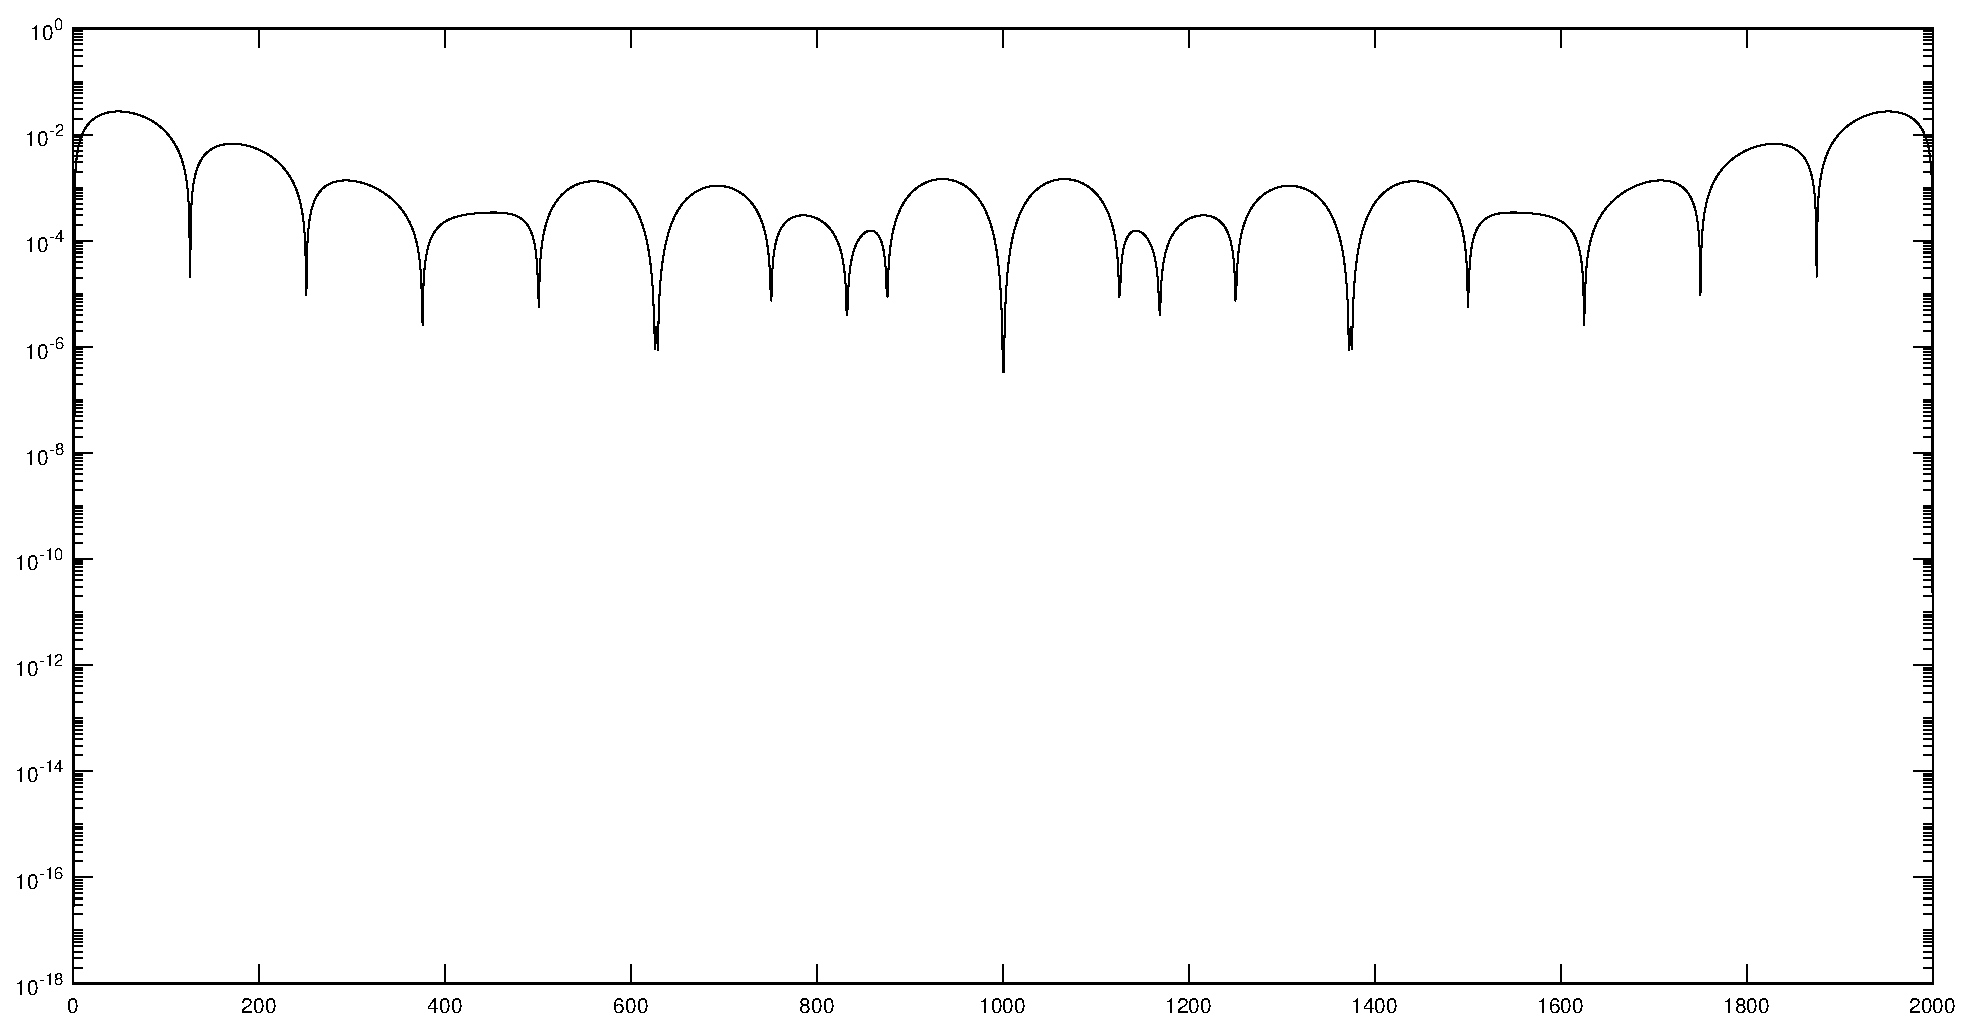
\includegraphics[width=0.85\textwidth]{1semilogy1}
			\caption{三次样条插值的逐点误差}  
			\label{1}  
		\end{figure} 
		\item[(c)](15分)使用不同的$n$,令$n = 2^4,2^5,...,2^{10}$重复上一问,取关于不同$n$的2000个等距点上的误差的最大值,用\textbf{loglog}图描述插值区间上最大误差值随$n$变化的情况(即横轴是$n$)。
		\begin{figure}[H]
			\centering
			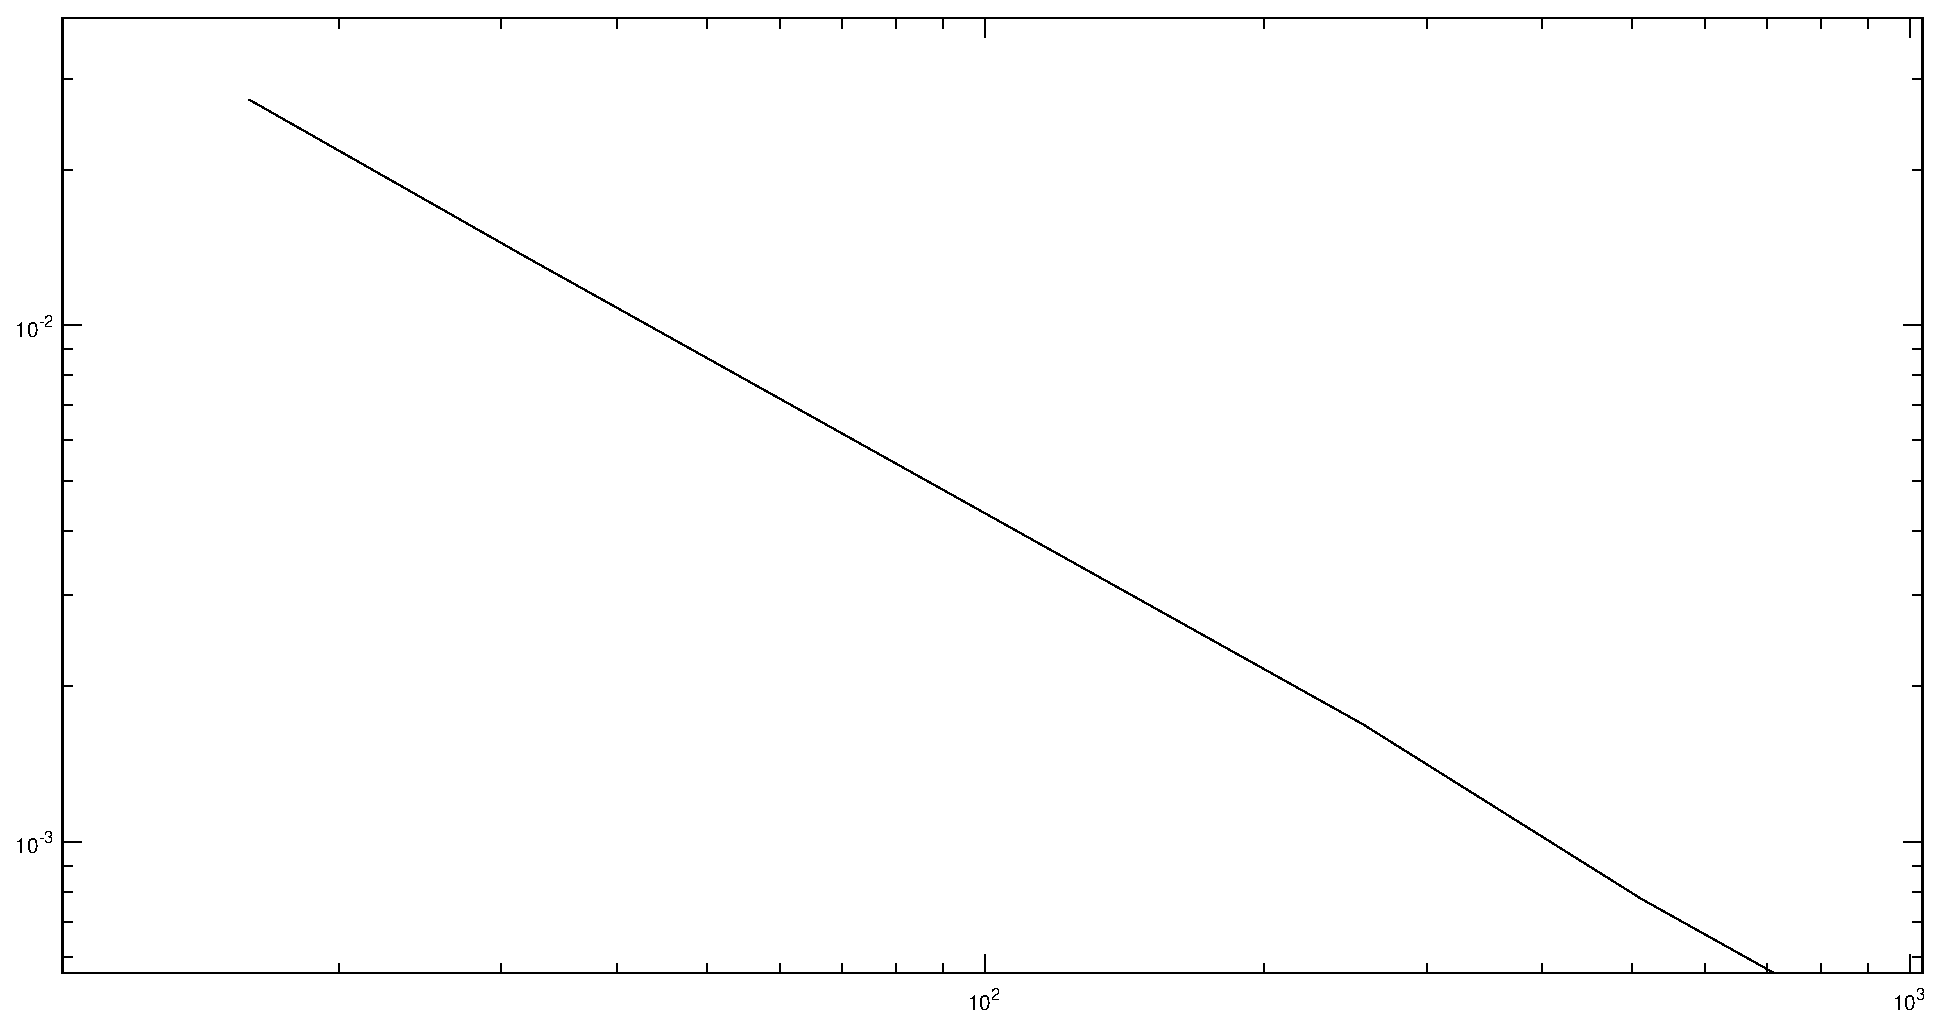
\includegraphics[width=0.85\textwidth]{1loglog1}
			\caption{最大误差随$n$的变化}  
			\label{2}  
		\end{figure} 
		\item[(d)](15分)针对周期边界条件,即假设三次样条函数满足$S^{'}(−1) = S^{'}(1)$和$S^{''}(−1) =S^{''}(1)$,重复完成上面三问中的要求。
		\par 推导过程:(*)号之前的推导不变\\
		由于$S_{i}^{''}\left(x_{i}\right)=S_{i-1}^{''}\left(x_{i}\right)$即$M_{0}=M_{n}$那么就有\\$$
		d_{n}=\lambda_{n} M_{1}+2 M_{n}+\mu_{n} M_{n-1}=\frac{6}{h_{n-1}+h_{0}}\left(\frac{y_{1}-y_{0}}{h_{0}}-\frac{y_{n}-y_{n-1}}{h_{n-1}}\right)$$
		其中$$\lambda_{n}=\frac{h_{n-1}}{h_{n-1}+h_{0}}, \quad \mu_{n}=1-\lambda_{n}$$\\
		得到如下线性方程组$$
		\left[\begin{array}{ccccc}
			2 & \lambda_{1} & & & \mu_{1} \\
			\mu_{2} & 2 & \lambda_{2} & & \\
			& \ddots & \ddots & \ddots & \\
			& & \mu_{n-1} & 2 & \lambda_{n-1} \\
			\lambda_{n} & & & \mu_{n} & 2
		\end{array}\right]\left[\begin{array}{c}
			M_{1} \\
			M_{2} \\
			\vdots \\
			M_{n-1} \\
			M_{n}
		\end{array}\right]=\left[\begin{array}{c}
			d_{1} \\
			d_{2} \\
			\vdots \\
			d_{n-1} \\
			d_{n}
		\end{array}\right]$$
		\begin{figure}[H]
			\centering
			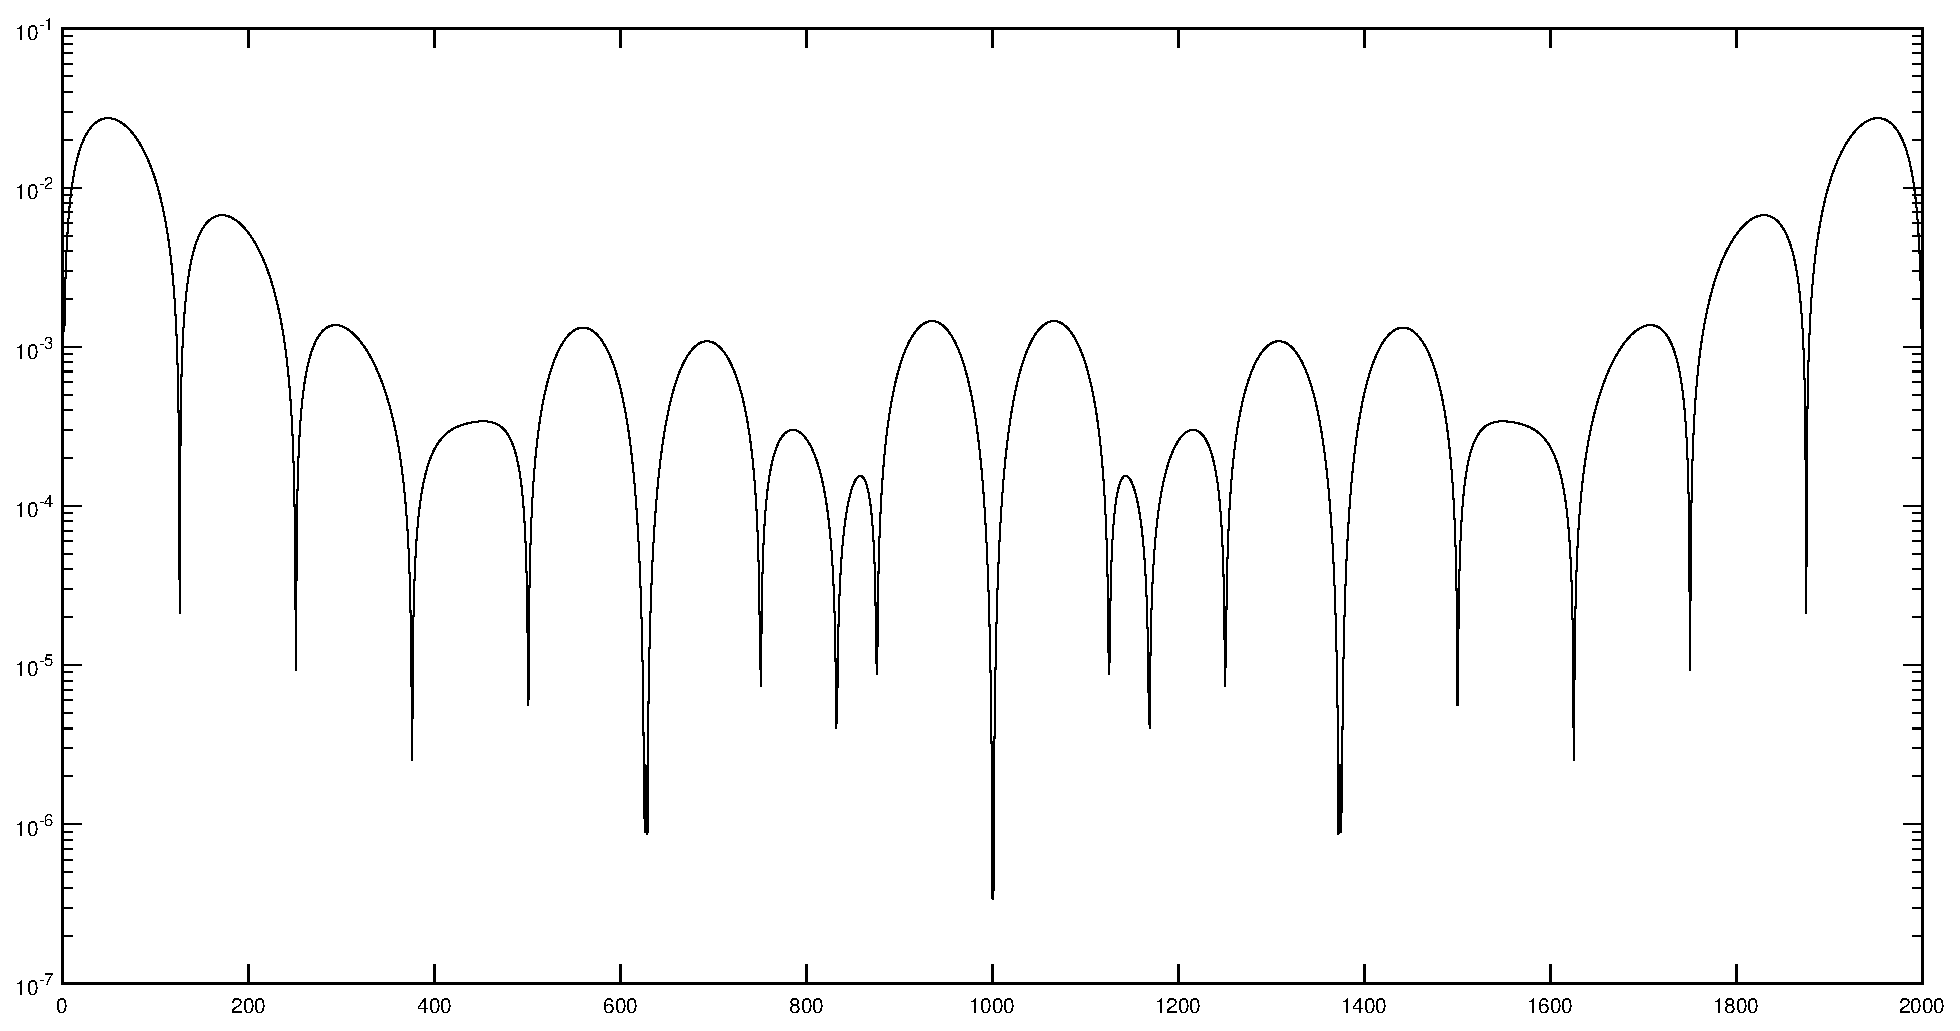
\includegraphics[width=0.85\textwidth]{1semilogy2}
			\caption{逐点误差}  
			\label{3}  
		\end{figure} 
		\begin{figure}[H]
			\centering
			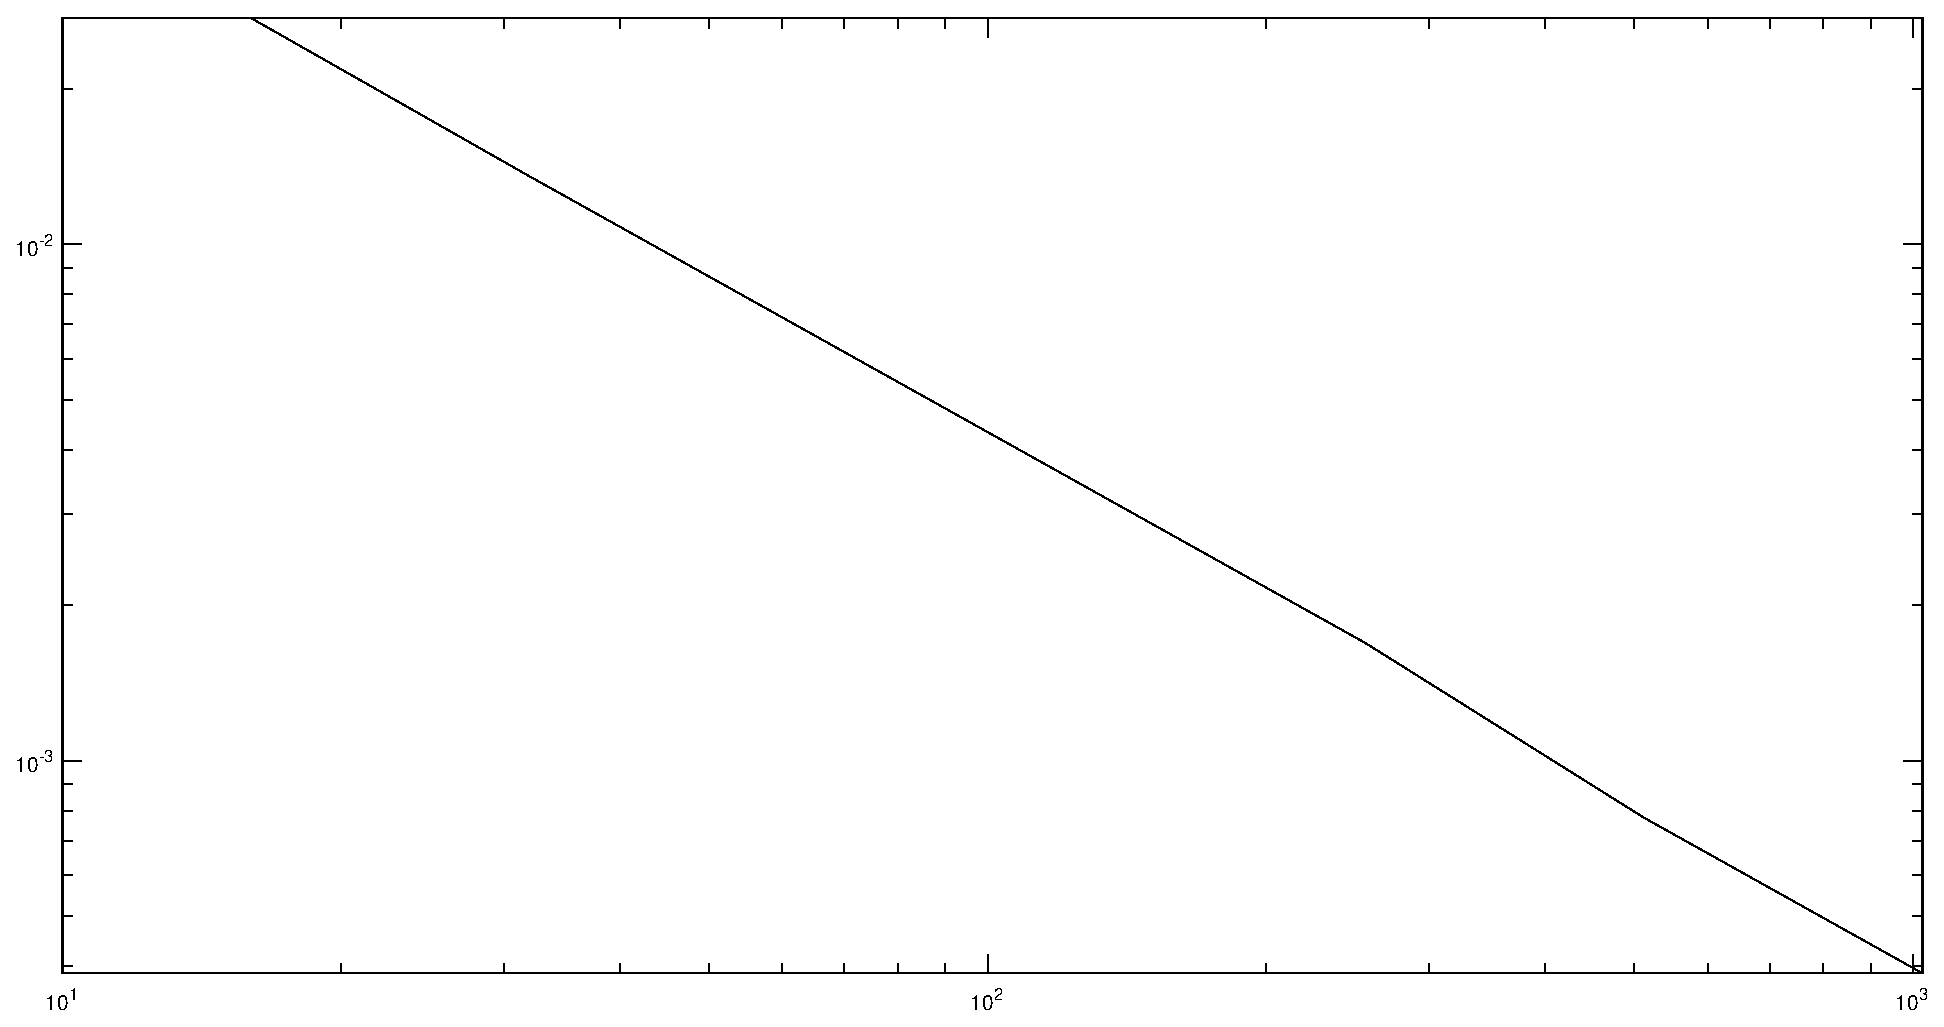
\includegraphics[width=0.85\textwidth]{1loglog2}
			\caption{最大误差随$n$的变化}  
			\label{4}  
		\end{figure} 
		(b)(c)的MATLAB代码如下
		\begin{lstlisting}[breaklines,frame=single]
			n=16;
			%计算插值点
			x=linspace(-1,1,n+1);
			y=zeros(1,n);
			for i=1:n+1
			y(i)=f(x(i));
			end
			%绘图初始化
			l=linspace(-1,1,2000);
			err=zeros(1,2000);
			st=zeros(1,2000);
			for i=1:2000
			st(i)=f(l(i));%真实值
			end
			%第二问
			for i=1:2000
			err(i)=abs(st(i)-myspine(l(i),n));
			end
			N=1:2000;
			semilogy(N,err);
			%第三问
			E=zeros(1,7);
			for i=1:7
			E(i)=2^(i+3);
			end
			merr=zeros(1,7);
			for j=1:7
			for i=1:2000
			err(i)=abs(st(i)-myspine(l(i),E(j)));
			end
			merr(j)=max(err);
			end
			loglog(E,merr);
			
			function M=getM(n,x,y)  %计算二阶导
			%x是插值点,y是对应的函数值(数组)
			for k=1:n     %计算h(i)
			h(k)=x(k+1)-x(k);
			end
			lambda=zeros(1,n-1);
			b=zeros(1,n-1);
			A=zeros(n+1,n+1);
			miu=lambda;
			for k=1:n-1    %计算miu和lambda
			lambda(k)=h(k+1)/(h(k)+h(k+1));
			miu(k)=1-lambda(k);
			end
			for k=1:n-1 %计算di
			b(k)=6/(h(k)+h(k+1))*((y(k+2)-y(k+1))/h(k+1)-(y(k+1)-y(k))/h(k));
			end
			d=zeros(1,n+1);
			d(1)=6/h(1)^2*(y(2)-y(1));
			d(n+1)=6/h(n)^2*(y(n)-y(n+1));
			for i=2:n
			d(i)=b(i-1);
			end
			d=d';
			A(1,2)=1;A(1,1)=2; %计算系数矩阵A
			A(n+1,n+1)=2;A(n+1,n)=1;
			for i=2:n
			A(i,i)=2;
			A(i,i-1)=miu(i-1);
			A(i,i+1)=lambda(i-1);
			end
			M=A\d;
			end
			
			function y=f(x)
			y=sin(4*x^2)+sin(4*x)^2;
			end
			
			function s=myspine(t,n)
			s=0;N=n;
			if t>1||t<-1
			fprintf('wrong input!\n');
			return;
			end
			x=linspace(-1,1,n+1);
			y=zeros(1,n);
			h=y;
			for i=1:n+1
			y(i)=f(x(i));
			end
			for k=1:n %计算h(i)
			h(k)=x(k+1)-x(k);
			end
			M=getM(N,x,y);
			%计算S(x)
			for i=1:n
			if t>=x(i)&&t<=x(i+1)
			break;
			end
			end
			s=((x(i+1)-t)^3*M(i)+(t-x(i))^3*M(i+1))/(6*h(i))+(y(i)*(x(i+1)-t)+y(i+1)*(t-x(i)))/h(i)-h(i)/6*(M(i)*(x(i+1)-t)+M(i+1)*(t-x(i)));
			end
		\end{lstlisting}
		(d)的MATLAB代码(主代码相同,不同之处在函数中)
		\begin{lstlisting}[breaklines,frame=single]
			n=16;
			x=linspace(-1,1,n+1);
			y=zeros(1,n);
			for i=1:n+1
			y(i)=f(x(i));
			end
			l=linspace(-1,1,2000);
			st=zeros(1,2000);
			p=zeros(1,2000);
			for i=1:2000
			st(i)=f(l(i));
			end
			for i=1:2000
			err(i)=abs(st(i)-myspine(l(i),n));
			end
			N=1:2000;
			semilogy(N,err);
			E=zeros(1,7);
			for i=1:7
			E(i)=2^(i+3);
			end
			merr=zeros(1,7);
			for j=1:7
			max=-1;
			for i=1:2000
			t=abs(st(i)-myspine(l(i),E(j)));
			if t>max
			max=t;
			end
			end
			merr(j)=max;
			end
			loglog(E,merr);
			function M1=getM(n,x,y)
			for k=1:n %计算h(i)
			h(k)=x(k+1)-x(k);
			end
			lambda=zeros(1,n);
			b=zeros(1,n);
			A=zeros(n,n);
			miu=lambda;
			for k=1:n-1 %计算miu和lambda
			lambda(k)=h(k+1)/(h(k)+h(k+1));
			miu(k)=1-lambda(k);
			end
			lambda(n)=h(1)/(h(n)+h(1));
			miu(n)=1-lambda(n);
			for k=1:n-1
			b(k)=6/(h(k)+h(k+1))*((y(k+2)-y(k+1))/h(k+1)-(y(k+1)-y(k))/h(k));
			end
			b(n)=6/(h(1)+h(n))*((y(2)-y(1))/h(1)-(y(1)-y(n))/h(1));
			b=b';
			A(1,n)=miu(1);A(1,1)=2;A(1,2)=lambda(1);
			A(n,1)=lambda(n);A(n,n)=2;A(n,n-1)=miu(n);
			for i=2:n-1
			A(i,i)=2;
			A(i,i-1)=miu(i);
			A(i,i+1)=lambda(i);
			end
			M=A\b;
			M1=[M(n),M']';
			end
			
			function y=f(x)
			y=sin(4*x^2)+sin(4*x)^2;
			end
			
			function s=myspine(t,n)
			s=0;
			x=linspace(-1,1,n+1);
			y=zeros(1,n);
			h=y;
			for i=1:n+1
			y(i)=f(x(i));
			end
			for k=1:n %计算h(i)
			h(k)=x(k+1)-x(k);
			end
			M=getM(N,x,y);
			%计算S(x)
			for i=1:n
			if t>=x(i)&&t<=x(i+1)
			break;
			end
			end
			s=((x(i+1)-t)^3*M(i)+(t-x(i))^3*M(i+1))/(6*h(i))+(y(i)*(x(i+1)-t)+y(i+1)*(t-x(i)))/h(i)-h(i)/6*(M(i)*(x(i+1)-t)+M(i+1)*(t-x(i)));
			end
		\end{lstlisting}
		\item[第二题] 本题深入讨论Newton插值公式的性质。
		\item[(a)](15分)对于一个光滑函数 $f(x)$, 证明若 $\left\{i_{0}, i_{1}, \ldots, i_{k}\right\}$ 是 $\{0,1, \ldots, k\}$ 的任意一个排列,则
		$$
		f\left[x_{0}, x_{1}, \ldots, x_{k}\right]=f\left[x_{i_{0}}, x_{i_{1}}, \ldots, x_{i_{k}}\right]
		$$
		证明:\\
		只需要证明$f\left[x_{0}, x_{1}, \ldots, x_{k}\right]$是关于$f(x_{i})$的线性组合。利用归纳法:\\
		显然有$$
		f\left[x_{0}, x_{1}\right]=\frac{f\left(x_{1}\right)-f\left(x_{0}\right)}{x_{1}-x_{0}}=\frac{f\left(x_{0}\right)}{x_{0}-x_{1}}+\frac{f\left(x_{1}\right)}{x_{1}-x_{0}}
		$$
		假设有$$
		f\left[x_{0}, x_{1}, \ldots, x_{n}\right]=\sum_{i=0}^{n}\frac{f(x_{i})}{\prod_{j\neq i}^{n}{(x_{j}-x_{i})}}$$
		$$
		f\left[x_{1}, x_{2}, \ldots, x_{n+1}\right]=\sum_{i=1}^{n+1}\frac{f(x_{i})}{\prod_{j\neq i}^{n+1}{(x_{j}-x_{i})}}
		$$
		那么当$k=n+1$的时候
		\begin{equation}
			\begin{aligned}
				&f\left[x_{0}, x_{1}, \ldots, x_{n+1}\right]=\frac{f\left[x_{1}, x_{2}, \ldots, x_{n+1}\right]-f\left[x_{0}, x_{1}, \ldots, x_{n}\right]}{x_{n+1}-x_{0}}\\
				&=\frac{1}{x_{n+1}-x_{0}}\left(\frac{f\left(x_{n+1}\right)}{\left(x_{n+1}-x_{1}\right)\left(x_{n+1}-x_{2}\right) \ldots\left(x_{n+1}-x_{n}\right)}+\frac{-f\left(x_{0}\right)}{\left(x_{0}-x_{1}\right)\left(x_{0}-x_{2}\right) \ldots\left(x_{0}-x_{n}\right)}\right)\\
				&+\sum_{j=1}^{n} \frac{f\left(x_{j}\right)}{x_{n+1}-x_{0}} \cdot \frac{\left(x_{j}-x_{0}\right)-\left(x_{j}-x_{n+1}\right)}{\left(x_{j}-x_{0}\right)\left(x_{j}-x_{1}\right) \ldots\left(x_{j}-x_{j-1}\right)\left(x_{j}-x_{j+1}\right) \ldots\left(x_{j}-x_{n+1}\right)}\\
				&=\sum_{j=0}^{n+1} \frac{f\left(x_{j}\right)}{\left(x_{j}-x_{0}\right)\left(x_{j}-x_{1}\right) \ldots\left(x_{j}-x_{j-1}\right)\left(x_{j}-x_{j+1}\right) \ldots\left(x_{j}-x_{n+1}\right)}\\
				&=\sum_{i=0}^{n+1}\frac{f(x_{i})}{\prod_{j\neq i}^{n+1}{(x_{j}-x_{i})}}
			\end{aligned}
		\end{equation}
		
		因此不论如何交换$x_{i}$的次序,差商都不变。\\
		证毕.
		\item[(b)](10分)课堂上我们提到了Chebyshev点
		$$
		x_{j}=\cos (j \pi / n) \quad j=0,1, \ldots, n
		$$
		以及使用Chebyshev点可以有效地克服Runge现象。写一个\textsc{Matlab}程序,令
		$n=2^{2}, 2^{3}, 2^{4}, \ldots, 2^{7}$, 按照从右到左的顺序(即 $j$ 从小到大的顺序)使用对应 的 $n+1$ 个Chebyshev点对定义在 $[-1,1]$ 上的Runge函数
		$$
		f(x)=\frac{1}{1+25 x^{2}}
		$$
		进行插值,并取2000个等距点上的误差的最大值,用\textbf{semilogy}图描述插值区间上最大误差值随 $n$ 变化的情况(即横轴是 $n$) 。
		\begin{figure}[H]
			\centering
			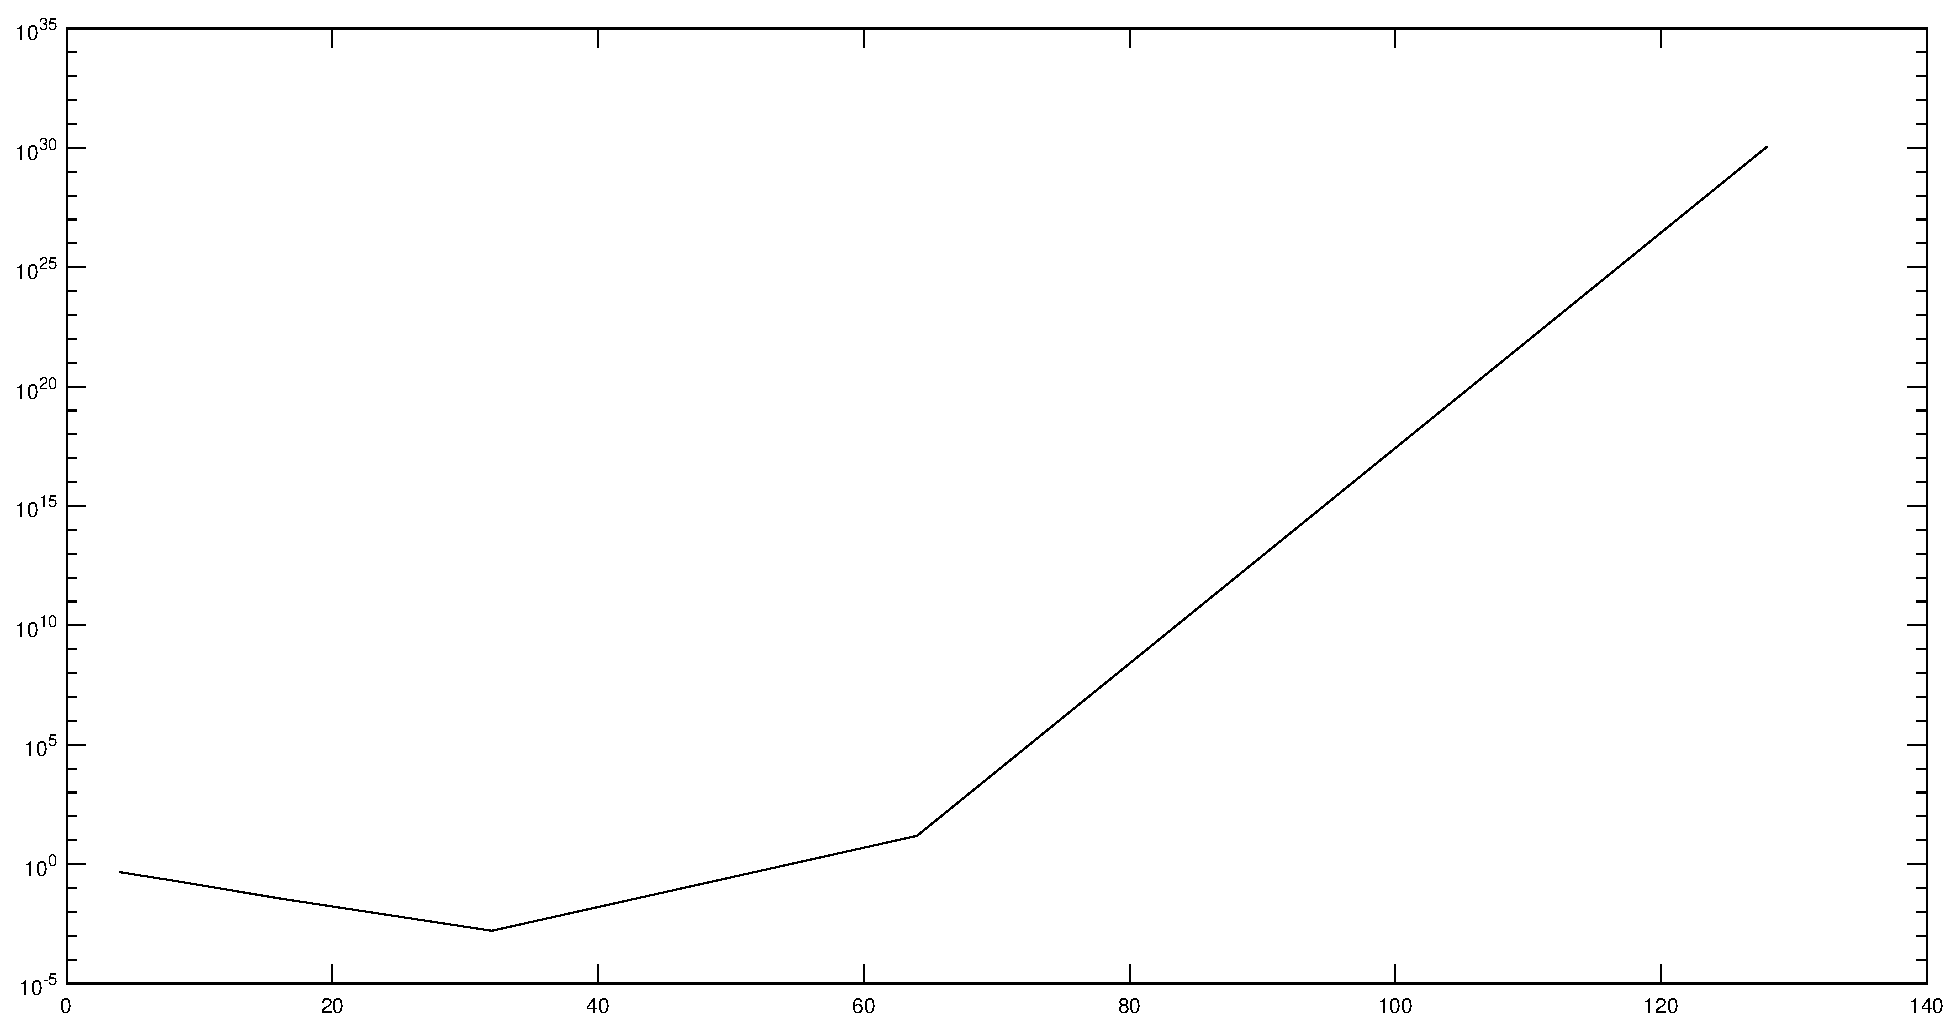
\includegraphics[width=\textwidth]{2semilogy1}
			\caption{最大误差随$n$的变化}  
			\label{5}  
		\end{figure} 

		\item[(c)](10分) 重复上一问,但使用随机数种子\textbf{rng(22)}和\textbf{randperm}函数来随机计算差商时插值点的使用顺序,取关于不同 $n$ 的2000个等距点上的误差的最大值,用\textbf{semilogy}图描述插值区间上最大误差值随 $n$ 变化的情况(即横轴是 $n$ )。
		\begin{figure}[H]
			\centering
			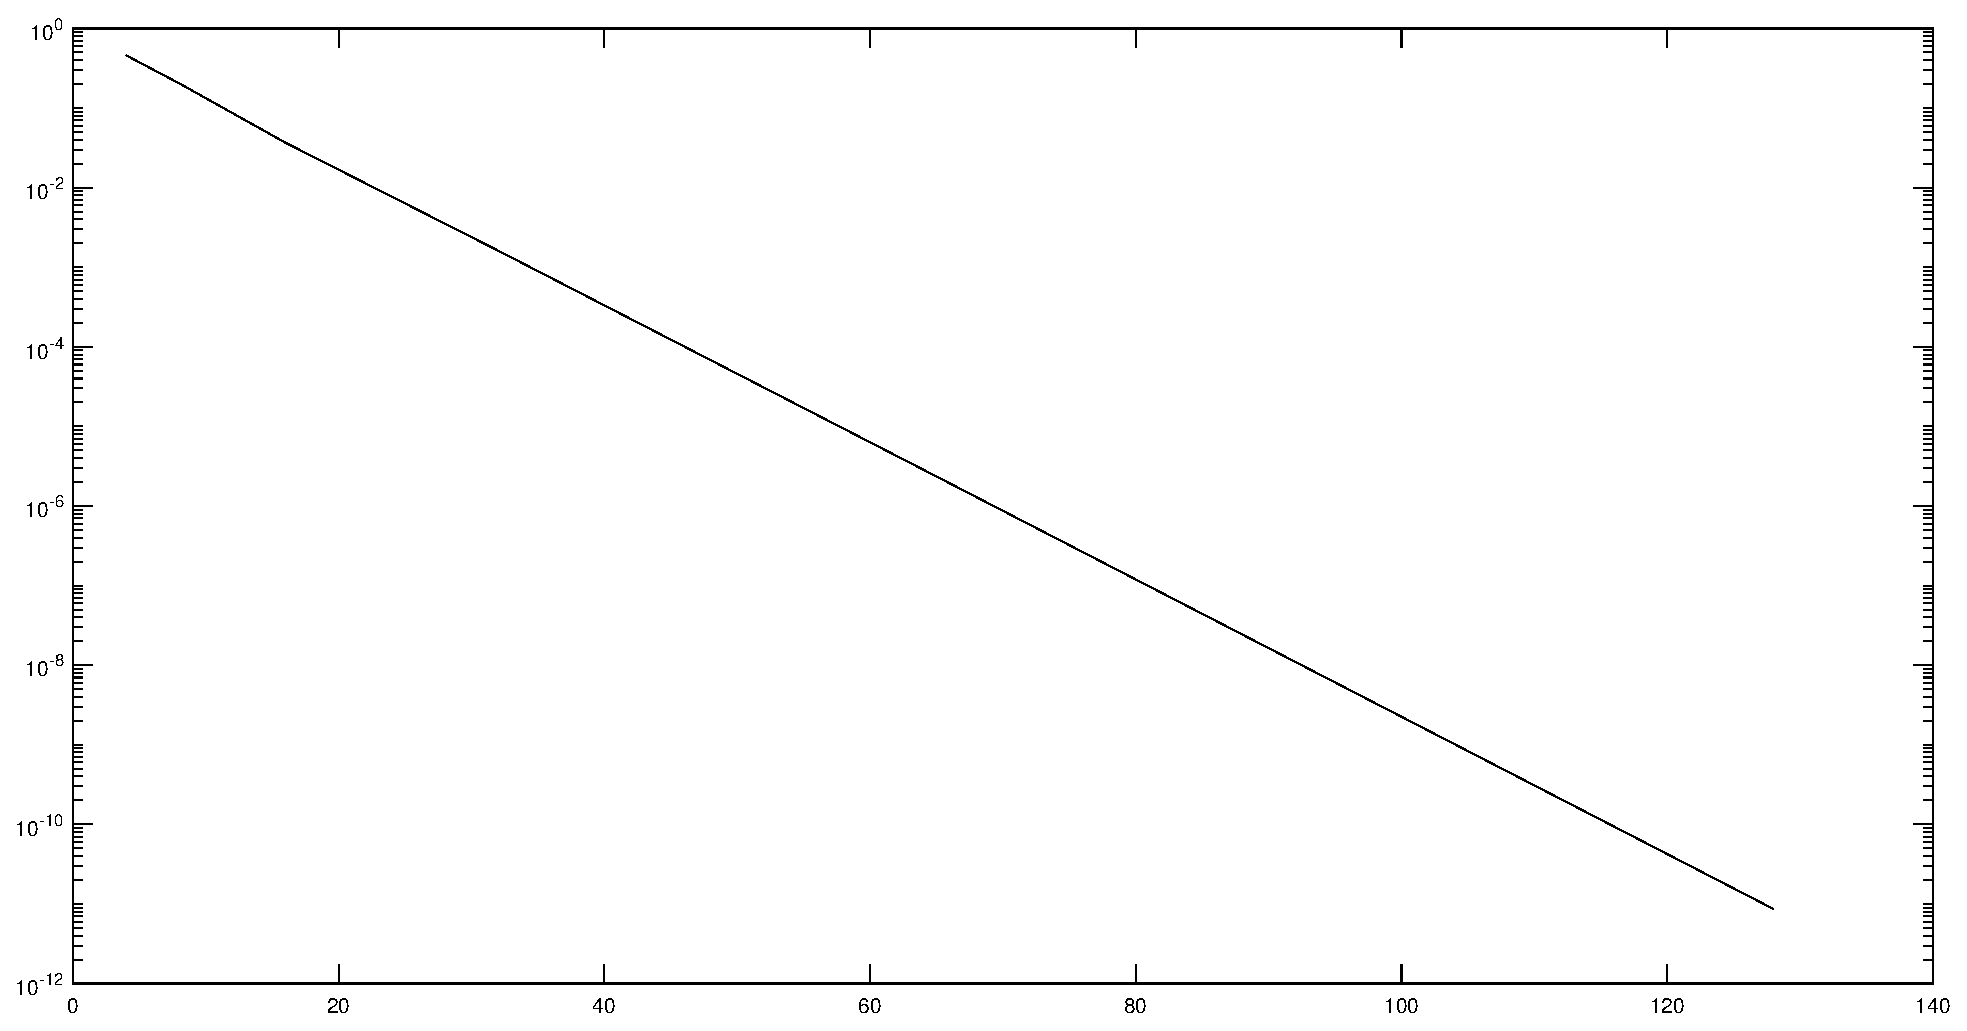
\includegraphics[width=\textwidth]{2semilogy2}
			\caption{最大误差随$n$的变化}  
			\label{6}  
		\end{figure} 		
		
		\item[(d)](10分)试着解释上面两小问中你观察到的不同现象产生的原因。注:此问答不出来也无妨。\\
		答:\par 
		\quad\quad 经过以上两小问,我们发现随机插入Chebyshev点的效果要比顺序插入好很多(不论是正序还是倒序)。更进一步地,在更换不同随机种子之后,得到的误差情况也不尽相同,但是他们都要比顺序插值的效果好很多。初步的分析:$$
		f(x)=f(x_{0})+(x-x_{0})f[x_{0},x_{1}]+\ldots+(x-x_{0})(x-x_{1})\ldots(x-x_{n-1})f[x_{0},x_{1},\ldots x_{n}]+R_{n}(x)$$
		$$R_{n}(x)=(x-x_{0})(x-x_{1})\ldots(x-x_{n})f[x,x_{0},x_{1},\ldots x_{n}]$$
		\quad\quad 而由(a)的推论知:不论如何交换$x_{i}$的次序,差商不变,因此顺序插值和Chebyshev插值的$R_{n}(x)$相同。同时注意到$N_{n}(x)$并不具有交换对称性,因此$N_{n}(x)$受插值顺序的影响。顺序插值时,$x_{0},x_{1}\ldots x_{n}$具有严格的大小关系,即使是Chebyshev点,在最后一个插值点$x_{n}$附近也会剧烈震荡,我认为主要是此时$x_{n}$点只有左侧有约束,因此右侧部分可能会过于“自由”;反观随机插值,最后插入的点往往在其他点列之间,因此两侧拥有更多的约束,所以得到的近似函数的性质也更好。
		
		\item[第三题]本题用于讨论周期函数的Lagrange插值方法。对于周期函数而言,多项式不再是最有效的基函数,而等距插值点也不再会出现Runge现象。逼近周期函数的基函 数通常选用三角函数或者复指数。同时注意对于周期函数而言,插值点数量和子区间个数相等。
		\item[(a)](10分)在 $[0,1]$ 上关于周期函数的基于等间距插值点 $x_{j}=\frac{j}{n}, j=0,1, \ldots$, $n-1$ 的Lagrange插值基函数为
		$$
		\ell_{k}(x)=\left\{\begin{array}{ll}
			\frac{(-1)^{k}}{n} \sin (n \pi x) \csc \left(\pi\left(x-x_{k}\right)\right) & \text { 若 } n \text { 为奇数 } \\
			\frac{(-1)^{k}}{n} \sin (n \pi x) \cot \left(\pi\left(x-x_{k}\right)\right) & \text { 若 } n \text { 为偶数 }
		\end{array}\right.
		$$
		证明对于 $n$ 分别为奇数和偶数的情况下
		$$
		\ell_{k}\left(x_{j}\right)=\left\{\begin{array}{ll}
			1 & k=j \\
			0 & k \neq j
		\end{array}\right.
		$$
		当$n$为奇数时$$
		\ell_{k}(x)=\frac{(-1)^{k} \sin (n \pi x)}{n\sin \left(\pi\left(x-x_{k}\right)\right)}
		$$
		如果$k\neq j$,那么$$
		\ell_{k}\left(x_{j}\right)=\frac{(-1)^{k} \sin (j \pi )}{n\sin \left(\pi\left(x_{j}-x_{k}\right)\right)}=0
		$$
		如果$k=j$,则$$
		\ell_{k}\left(x_{j}\right)=\lim_{x\to x_{j}}\frac{(-1)^{k} \sin (n \pi x)}{n\sin \left(\pi\left(x-x_{k}\right)\right)}=\lim_{x\to x_{j}}\frac{(-1)^{k} \cos (n \pi x)}{\cos \left(\pi\left(x-x_{k}\right)\right)}=(-1)^{k+j}=1 $$
		如果$n$为偶数$$
		\ell_{k}(x)=\frac{(-1)^{k}\sin( n\pi x)\cos(\pi (x-x_{k}))}{n\sin(\pi (x-x_{k}))}
		$$如果$k\neq j$ $$
		\ell_{k}\left(x_{j}\right)=\frac{(-1)^{k}\sin( j\pi )\cos(\pi (x_{j}-x_{k}))}{n\sin(\pi (x_{j}-x_{k}))}=0
		$$如果$k=j$ 
		
		\begin{equation}
			\begin{aligned}
				\ell_{k}\left(x_{j}\right)&=\lim_{x\to x_{j}}\frac{(-1)^{k}\sin( n\pi x)\cos(\pi (x-x_{k}))}{n\sin(\pi (x-x_{k}))}\\
				&=\lim_{x\to x_{j}}\frac{(-1)^{k}\sin( n\pi x)}{n\sin(\pi (x-x_{k}))}\\&=\lim_{x\to x_{j}}\frac{(-1)^{k}\cos( n\pi x)}{\cos(\pi (x-x_{k}))}\\&=(-1)^{k+j}=1
			\end{aligned}			
		\end{equation}

		
		
		\item[(b)](10分)用上述对应于 $n$ 为偶数的Lagrange基函数构造Lagrange插值多项式, 并用 $n=2^{6}$ 个点对周期函数 $f(x)=\sin (2 \pi x) e^{\cos (2 \pi x)}$ 在 $[0,1]$ 上进行插值。取1000个 等距点上的误差,用\textbf{semilogy}图描述插值区间上误差值随 $x$ 变化的情况(即 横轴是 $x$ )。
		\begin{figure}[H]
			\centering
			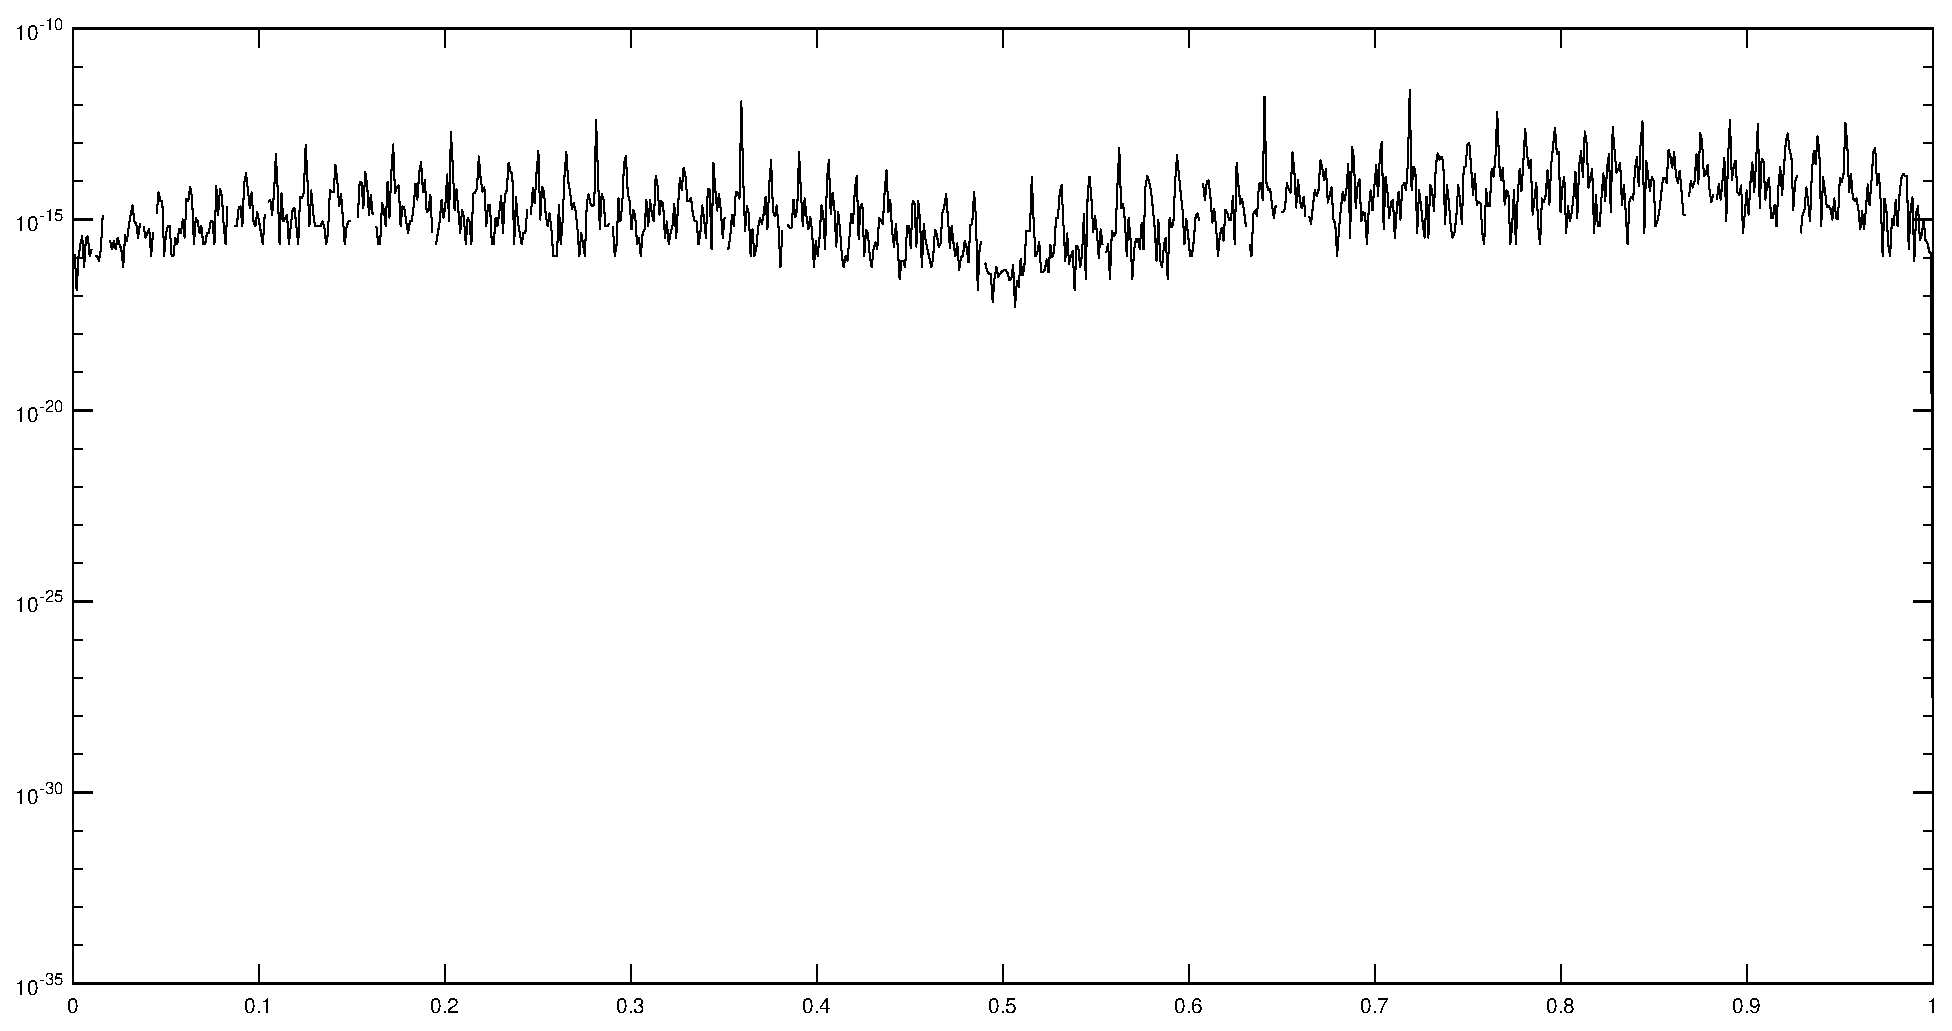
\includegraphics[width=\textwidth]{3semilogy}
			\caption{误差随$x$的变化}  
			\label{7}  
		\end{figure} 
	MATLAB程序如下:
		\begin{lstlisting}[breaklines,frame=single]
			n=2^6;
			x=zeros(n,1);
			for i=1:n
			x(i)=(i-1)/n;
			end
			y=zeros(n,1);
			l=zeros(n,1);
			for i=1:n
			y(i)=f(x(i));
			end
			X=linspace(0,1,1000);
			T=zeros(1000,1);
			Y=T;
			err=zeros(1000,1);
			for i=1:1000
			T(i)=f(X(i));
			Y(i)=lagrange(X(i),x,y,n);
			err(i)=abs(T(i)-Y(i));
			end
			%绘图
			semilogy(X,err);
	
			function ans=lagrange(t,x,y,n)
			ans=0;
			for k=1:n
			l(k)=(-1)^(k-1)*sin(n*pi*t)*cot(pi*(t-x(k)))/n;
			ans=ans+y(k)*l(k);
			end
			end
			
			function y=f(x)
			y=sin(2*pi*x)*exp(cos(2*pi*x));
			end
		\end{lstlisting}
	\end{enumerate}
	\begin{enumerate}
		
		\item[第四题](10分) \textbf{写程序}完成课本59页第7题,并计算出你的拟合函数对比所给数据点的误差的2-范数。\\
		解:\\
			\text{a=2.52621737591824}\\
			\text{b=0.44739055018957}\\
			\text{误差的2-范数为0.00571447705504}\\
			对实验数据的预处理为:
			令$$
			Q=\sum (x_{i}-(a+bx_{i})y_{i})^{2}
			$$并有$$
			\frac{\partial Q}{\partial a}=\sum (x_{i}-y_{i}(a+bx_{i}))y_{i}=0
			$$ $$
			\frac{\partial Q}{\partial b}=\sum (x_{i}-y_{i}(a+bx_{i}))x_{i}y_{i}=0
			$$解之即得到$a,b$\\
			MATLAB程序如下
		\begin{lstlisting}[breaklines,frame=single]
			syms a b;
			x0=[2.1 2.5 2.8 3.2];
			y0=[0.6087 0.6849 0.7368 0.8111];
			eq1=0;eq2=0;
			for i=1:4
			eq1=eq1+(x0(i)-y0(i)*(a+b*x0(i)))*y0(i);
			eq2=eq2+(x0(i)-y0(i)*(a+b*x0(i)))*y0(i)*x0(i);
			end
			s=solve(eq1,eq2,a,b);
			fprintf('a=%.14f\nb=%.14f\n',s.a,s.b);
			%计算误差2-范数
			err=0;
			for i=1:4
			err=err+(y0(i)-x0(i)/(s.a+s.b*x0(i)))^2;
			end
			err=err^0.5;
			fprintf('误差的2-范数为%.14f\n',err);
		\end{lstlisting}
	\end{enumerate}
\end{document}
